% Figure -- whole-set vs designable diversity over training. Replaces the old
% 400K/700K/1.0M snapshot Table 6.8. \input{} from Ch6 sec:proteina-anatomy.
\begin{figure}[tbp]
\centering
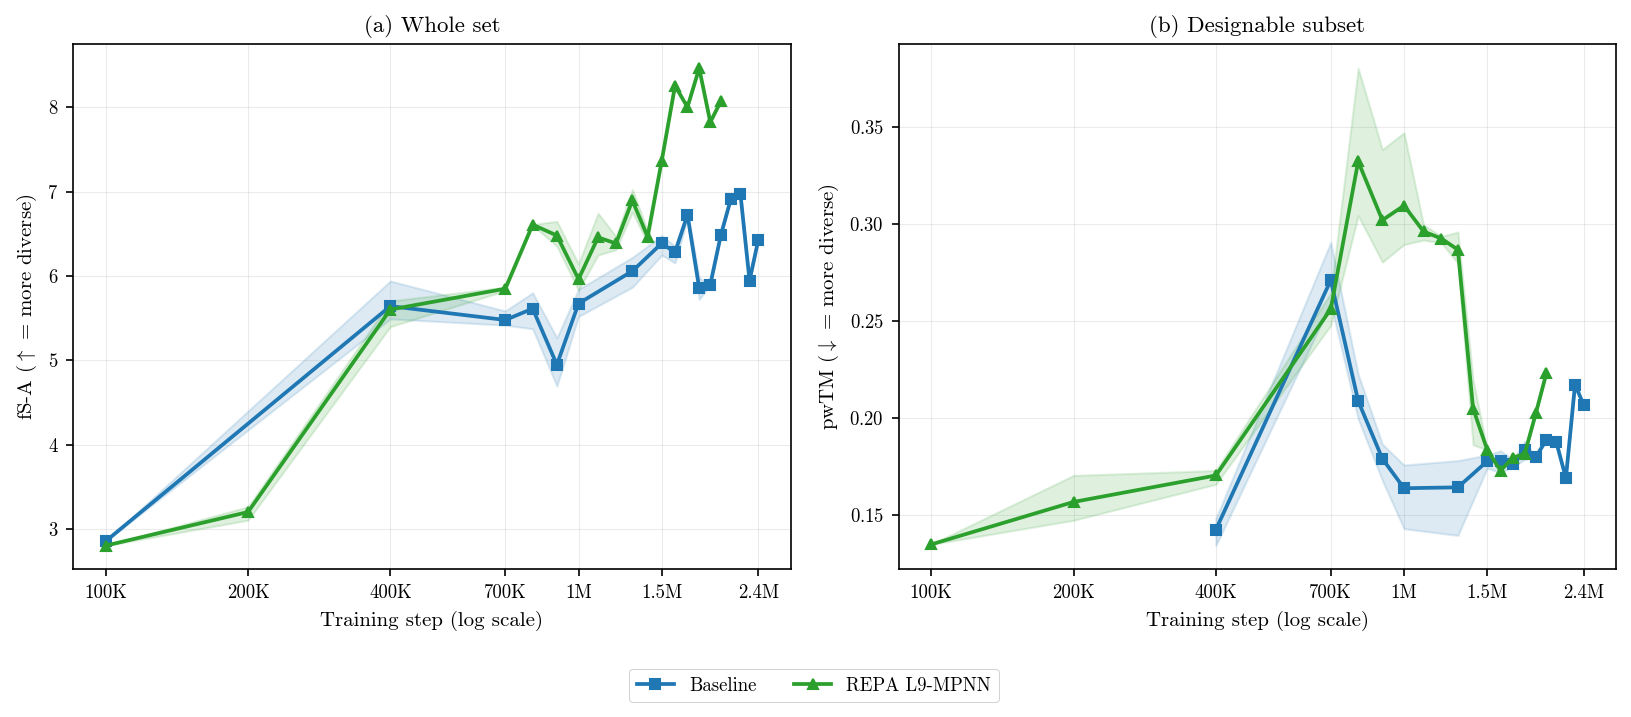
\includegraphics[width=\textwidth]{figures/fig5_diversity_trend.png}
\caption{\textbf{Over training, REPA's whole set grows more diverse than the baseline while its designable subset concentrates.} (a) Whole-set fold spread (fS-A; higher\,=\,more diverse): REPA climbs above the baseline. (b) Designable-subset pwTM (lower\,=\,more diverse): REPA rises above the baseline, i.e.\ more concentrated. This tracks one variant across training; Table~\ref{tab:proteina-13m} makes the same point at a fixed checkpoint across all variants. (Baseline vs.\ the representative variant, REPA-L9-MPNN.)}
\label{fig:proteina-diversity-trend}
\end{figure}
